\documentclass{beamer}
\usepackage[utf8]{inputenc}

\usetheme{Madrid}
\usecolortheme{default}
\usepackage{amsmath,amssymb,amsfonts,amsthm}
\usepackage{txfonts}
\usepackage{tkz-euclide}
\usepackage{listings}
\usepackage{adjustbox}
\usepackage{array}
\usepackage{tabularx}
\usepackage{gvv}
\usepackage{lmodern}
\usepackage{circuitikz}
\usepackage{tikz}
\usepackage{graphicx}

\setbeamertemplate{page number in head/foot}[totalframenumber]

\usepackage{tcolorbox}
\tcbuselibrary{minted,breakable,xparse,skins}



\definecolor{bg}{gray}{0.95}
\DeclareTCBListing{mintedbox}{O{}m!O{}}{%
	breakable=true,
	listing engine=minted,
	listing only,
	minted language=#2,
	minted style=default,
	minted options={%
		linenos,
		gobble=0,
		breaklines=true,
		breakafter=,,
		fontsize=\small,
		numbersep=8pt,
		#1},
	boxsep=0pt,
	left skip=0pt,
	right skip=0pt,
	left=25pt,
	right=0pt,
	top=3pt,
	bottom=3pt,
	arc=5pt,
	leftrule=0pt,
	rightrule=0pt,
	bottomrule=2pt,
	toprule=2pt,
	colback=bg,
	colframe=orange!70,
	enhanced,
	overlay={%
		\begin{tcbclipinterior}
			\fill[orange!20!white] (frame.south west) rectangle ([xshift=20pt]frame.north west);
	\end{tcbclipinterior}},
	#3,
}
\lstset{
	language=C,
	basicstyle=\ttfamily\small,
	keywordstyle=\color{blue},
	stringstyle=\color{orange},
	commentstyle=\color{green!60!black},
	numbers=left,
	numberstyle=\tiny\color{gray},
	breaklines=true,
	showstringspaces=false,
}
%------------------------------------------------------------
%This block of code defines the information to appear in the
%Title page
\title %optional
{5.2.49}
%\subtitle{A short story}

\author % (optional)
{RAVULA SHASHANK REDDY - EE25BTECH11047}

 \begin{document}
	
	
	\frame{\titlepage}
	\begin{frame}{Question}
    Solve the system of equations using matrices:
\begin{align*}
3x - y - 2z &= 2, \\
2y - z &= -1, \\
3x - 5y &= 3.
\end{align*}

\end{frame}
\begin{frame}{Solution}

Given:
\begin{align}
\myvec{3\\-1\\-2}^{T}\vec{x}&=2,\\
\myvec{0\\2\\-1}^{T}\vec{x}&=-1,\\
\myvec{3\\-5\\0}^{T}\vec{x}&=3\\
\myvec{3 & -1 & -2  \\
0 & 2 & -1  \\
3 & -5 & 0 } \vec{x} &= \myvec{2 \\ -1 \\ 3}
\end{align}
\end{frame}
\begin{frame}{Solution}
\begin{align}
R_3\rightarrow R_3-R_1 &\Rightarrow
\myvec{3 & -1 & -2 & 2 \\
0 & 2 & -1 & -1 \\
0 & -4 & 2 & 1}
\end{align}
\begin{align}
R_2\rightarrow \tfrac{1}{2}R_2 &\Rightarrow
\myvec{3 & -1 & -2 & 2 \\
0 & 1 & -\tfrac{1}{2} & -\tfrac{1}{2} \\
0 & -4 & 2 & 1}
\end{align}
\begin{align}
R_1\rightarrow R_1+R_2,\quad R_3\rightarrow R_3+4R_2 &\Rightarrow
\myvec{3 & 0 & -\tfrac{5}{2} & \tfrac{3}{2} \\
0 & 1 & -\tfrac{1}{2} & -\tfrac{1}{2} \\
0 & 0 & 0 & -1}
\\[6pt]
&\implies 0=-1
\end{align}

\[
\text{System inconsistent}\quad\Rightarrow\quad\boxed{\text{No solution}}
\]

    
\end{frame}
\begin{frame}[fragile]
\frametitle{C Code}
\begin{lstlisting}
    #include <stdio.h>
#include <math.h>

#define N 3

int main() {
    int i, j, k;
    double A[N][N+1] = {
        {3, -1, -2, 2},
        {0,  2, -1, -1},
        {3, -5,  0, 3}
    };

    // Forward elimination
    for (i = 0; i < N; i++) {
        // Pivot should not be zero (no pivoting added here for simplicity)
        if (fabs(A[i][i]) < 1e-9) continue;
\end{lstlisting}
\end{frame}
\begin{frame}[fragile]
\frametitle{C Code}
\begin{lstlisting}
        // Normalize row
        double div = A[i][i];
        for (j = i; j <= N; j++) {
            A[i][j] /= div;
        }

        // Eliminate other rows
        for (k = 0; k < N; k++) {
            if (k == i) continue;
            double factor = A[k][i];
            for (j = i; j <= N; j++) {
                A[k][j] -= factor * A[i][j];
            }
        }
    }

    // Check for inconsistency
    int inconsistent = 0;
    \end{lstlisting}
\end{frame}
\begin{frame}[fragile]
\frametitle{C Code}
\begin{lstlisting}
    for (i = 0; i < N; i++) {
        int allZero = 1;
        for (j = 0; j < N; j++) {
            if (fabs(A[i][j]) > 1e-9) {
                allZero = 0;
                break;
            }
        }
        if (allZero && fabs(A[i][N]) > 1e-9) {
            inconsistent = 1;
            break;
        }
    }
\end{lstlisting}
\end{frame}
\begin{frame}[fragile]
\frametitle{C Code}
\begin{lstlisting}
    if (inconsistent) {
        printf("System is inconsistent -> No solution\\n");
    } else {
        printf("Solution:\\n");
        for (i = 0; i < N; i++) {
            printf("x%d = %lf\\n", i+1, A[i][N]);
        }
    }

    return 0;
}
\end{lstlisting}
\end{frame}
\begin{frame}[fragile]
\frametitle{Python Direct}
\begin{lstlisting}
import numpy as np
import matplotlib.pyplot as plt

# local imports as you asked
import libs.line.funcs as linefuncs
import libs.triangle.funcs as trifuncs

# Coefficients of the system Ax=b
A = np.array([
    [3, -1, -2],
    [0,  2, -1],
    [3, -5,  0]
], dtype=float)

b = np.array([2, -1, 3], dtype=float)

# Check consistency via rank
rankA = np.linalg.matrix_rank(A)
\end{lstlisting}
\end{frame}
\begin{frame}[fragile]
\frametitle{Python Direct}
\begin{lstlisting}
rankAb = np.linalg.matrix_rank(np.c_[A, b])

print("Rank(A) =", rankA)
print("Rank([A|b]) =", rankAb)

if rankA != rankAb:
    print("System is inconsistent -> No solution")

# --- Plot the planes ---
fig = plt.figure()
ax = fig.add_subplot(111, projection='3d')
\end{lstlisting}
\end{frame}
\begin{frame}[fragile]
\frametitle{Python Direct}
\begin{lstlisting}
# Create a meshgrid for x,y
x_vals = np.linspace(-5, 5, 50)
y_vals = np.linspace(-5, 5, 50)
X, Y = np.meshgrid(x_vals, y_vals)

# Equation 1: 3x - y - 2z = 2 -> z = (3x - y - 2)/2
Z1 = (3*X - Y - 2)/2

# Equation 2: 2y - z = -1 -> z = 2y + 1
Z2 = 2*Y + 1

# Equation 3: 3x - 5y = 3 -> (no z term, it's a vertical plane)
# So plot separately
Z3 = np.linspace(-5, 5, 50)
X3, Z3m = np.meshgrid(x_vals, Z3)
Y3 = (3*X3 - 3)/5
\end{lstlisting}
\end{frame}
\begin{frame}[fragile]
\frametitle{Python Direct}
\begin{lstlisting}
# Plot the planes
ax.plot_surface(X, Y, Z1, alpha=0.5, color='red', label='Plane 1')
ax.plot_surface(X, Y, Z2, alpha=0.5, color='blue', label='Plane 2')
ax.plot_surface(X3, Y3, Z3m, alpha=0.5, color='green', label='Plane 3')

# Labels
ax.set_xlabel("x")
ax.set_ylabel("y")
ax.set_zlabel("z")
ax.set_title("Three Planes (Inconsistent System)")

plt.show()
\end{lstlisting}
\end{frame}
\begin{frame}[fragile]
\frametitle{Python Shared}
\begin{lstlisting}
import ctypes
import numpy as np

# Load the shared library
lib = ctypes.CDLL("./libgauss.so")

# Function signature: int solve_system(double *A_in, double *x_out)
lib.solve_system.argtypes = [ctypes.POINTER(ctypes.c_double),
                             ctypes.POINTER(ctypes.c_double)]
lib.solve_system.restype = ctypes.c_int

# Input augmented matrix [A|b]
A = np.array([
    [3, -1, -2,  2],   # 3x - y - 2z = 2
    [0,  2, -1, -1],   # 2y - z = -1
    [3, -5,  0,  3]    # 3x - 5y = 3
], dtype=np.float64)
\end{lstlisting}
\end{frame}
\begin{frame}[fragile]
\frametitle{Python Shared}
\begin{lstlisting}
A_flat = A.flatten()
x_out = np.zeros(3, dtype=np.float64)

# Call the C function
status = lib.solve_system(A_flat.ctypes.data_as(ctypes.POINTER(ctypes.c_double)),
                          x_out.ctypes.data_as(ctypes.POINTER(ctypes.c_double)))

if status == 1:
    print("System is inconsistent -> No solution")
else:
    print("Solution:", x_out)

\end{lstlisting}
\end{frame}
\begin{frame}{Plot}
\begin{figure}
    \centering
    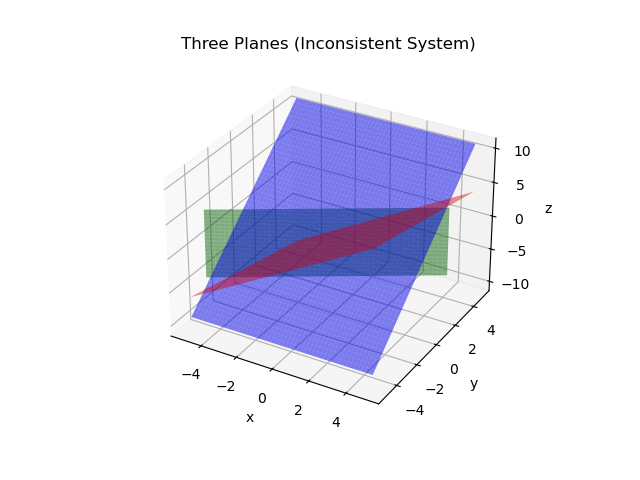
\includegraphics[width=0.75\linewidth]{figs/fig1.png}
    \caption{}
    \label{fig:placeholder}
\end{figure}
\end{frame}
\end{document}